\section{Introduction}

\subsection{Course Objectives}
The objective of this project was to design and manufacture a Search and Rescue Robot (SaRR) capable of navigating an obstacle course in order to deliver a first aid kit (the "medkit") to a trapped victim. The obstacle course consists of a pylon, a 12" high wall, and a chute. The first portion of the course involves picking up the 4" x 4" x 4", 3 pound medkit, navigating around the pylon, and approaching the wall using open-loop drive control via a remote controller. However, the rest of the course must be completed autonomously by the SaRR. First, the SaRR must cross a wall (one foot tall by three feet wide and consisting of two equally sized steps). The SaRR then approaches and navigates through a 3' chute with sharp bends without hitting the sides. Finally, the SaRR must acquire and track a light signal in order to deposit the med-kit in a 4" deep basket, mounted on top of a 4" block of wood that has a light source embedded in its frame. The timeline for meeting each of these objectives is given in Section 3. 


\subsection{Philosophy and Research}
The driving philosophy in the design of DynaSaRR was to build a robust, innovative robot able to surmount all the obstacles in the course. Additional consideration was given to places where previous SaRRs tended to fail.

The SaRRchaeologists spent roughly 5 hours researching, and 10-15 hours discussing potential designs before deciding upon the outline of what eventually became the design that can be seen in Figure 1. Much of this time was focused on designing a wall traversal mechanism, as this appeared to be the biggest challenge on the course. The SaRRchaeologists wanted to create a unique and creative design, and so decided to veer away from robots that relied on oversized wheels as a means of wall traversal. The robots that did not fall into that category all had some sort of mechanism that was meant to pull the front of the robot over the steps (4-spoked front wheels, four bar linkages, and grappling hooks).

Approximately 1 hour was spent studying the robots with grappling hooks. While there were successful robots that utilized this method, ultimately it did not seem like a reliable method of wall traversal. What's more, it was determined that calculating the proper trajectory for the the grappling hook to fire would be unnecessarily complicated. Finally, robots utilizing this method had trouble keeping the medkit secured during the wall traversal.

Only one robot utilized a four bar linkage, and while it worked smoothly and successfully, further exploration led the SaRRchaeologists to conclude that this method would result in a prohibitively heavy robot, had the potential for many mechanical failures, and left no recourse in the event of a failure during the wall traversal. 

The SaRRchaeologists noted that the 4-spoked front wheels appeared frequently on various robots, and tended to succeed more often than not. However, the logic behind this method appeared to be to spin the wheels at a high rate until the robot either got stuck or made it over the wall. The SaRRchaeologists wanted more control over the process and so adapted the 4-spoked wheels to what ultimately became the lifting arm. Finally, the SaRRchaeologists noticed that a considerable number of robots (roughly 5-7) would stall at the top of the wall. As a result, the driving wheels were designed with a large enough diameter to be in contact with two surfaces as the robot climbed the wall--first the ground and top corner of the first step, and then the top of the first step and top corner of the wall. Second, a hook was placed on the lifting arm at the stall point so that the arm could continue spinning, catch onto the wall, and push DynaSaRR off once it reached the top of the wall. The lifting arm geometry--the length of each side, hook placement, and mounting on the frame--was carefully designed by building a cardboard prototype and iteratively moving and reshaping the arms until they pulled the chassis smoothly over the wall. As a result, each step in the wall traversal was designed for separately, with the intent of making it easily replicable with autonomous code. The results of this design process are shown in Fig. \ref{fig:LiftingArm}.
\begin{figure}[ht]
    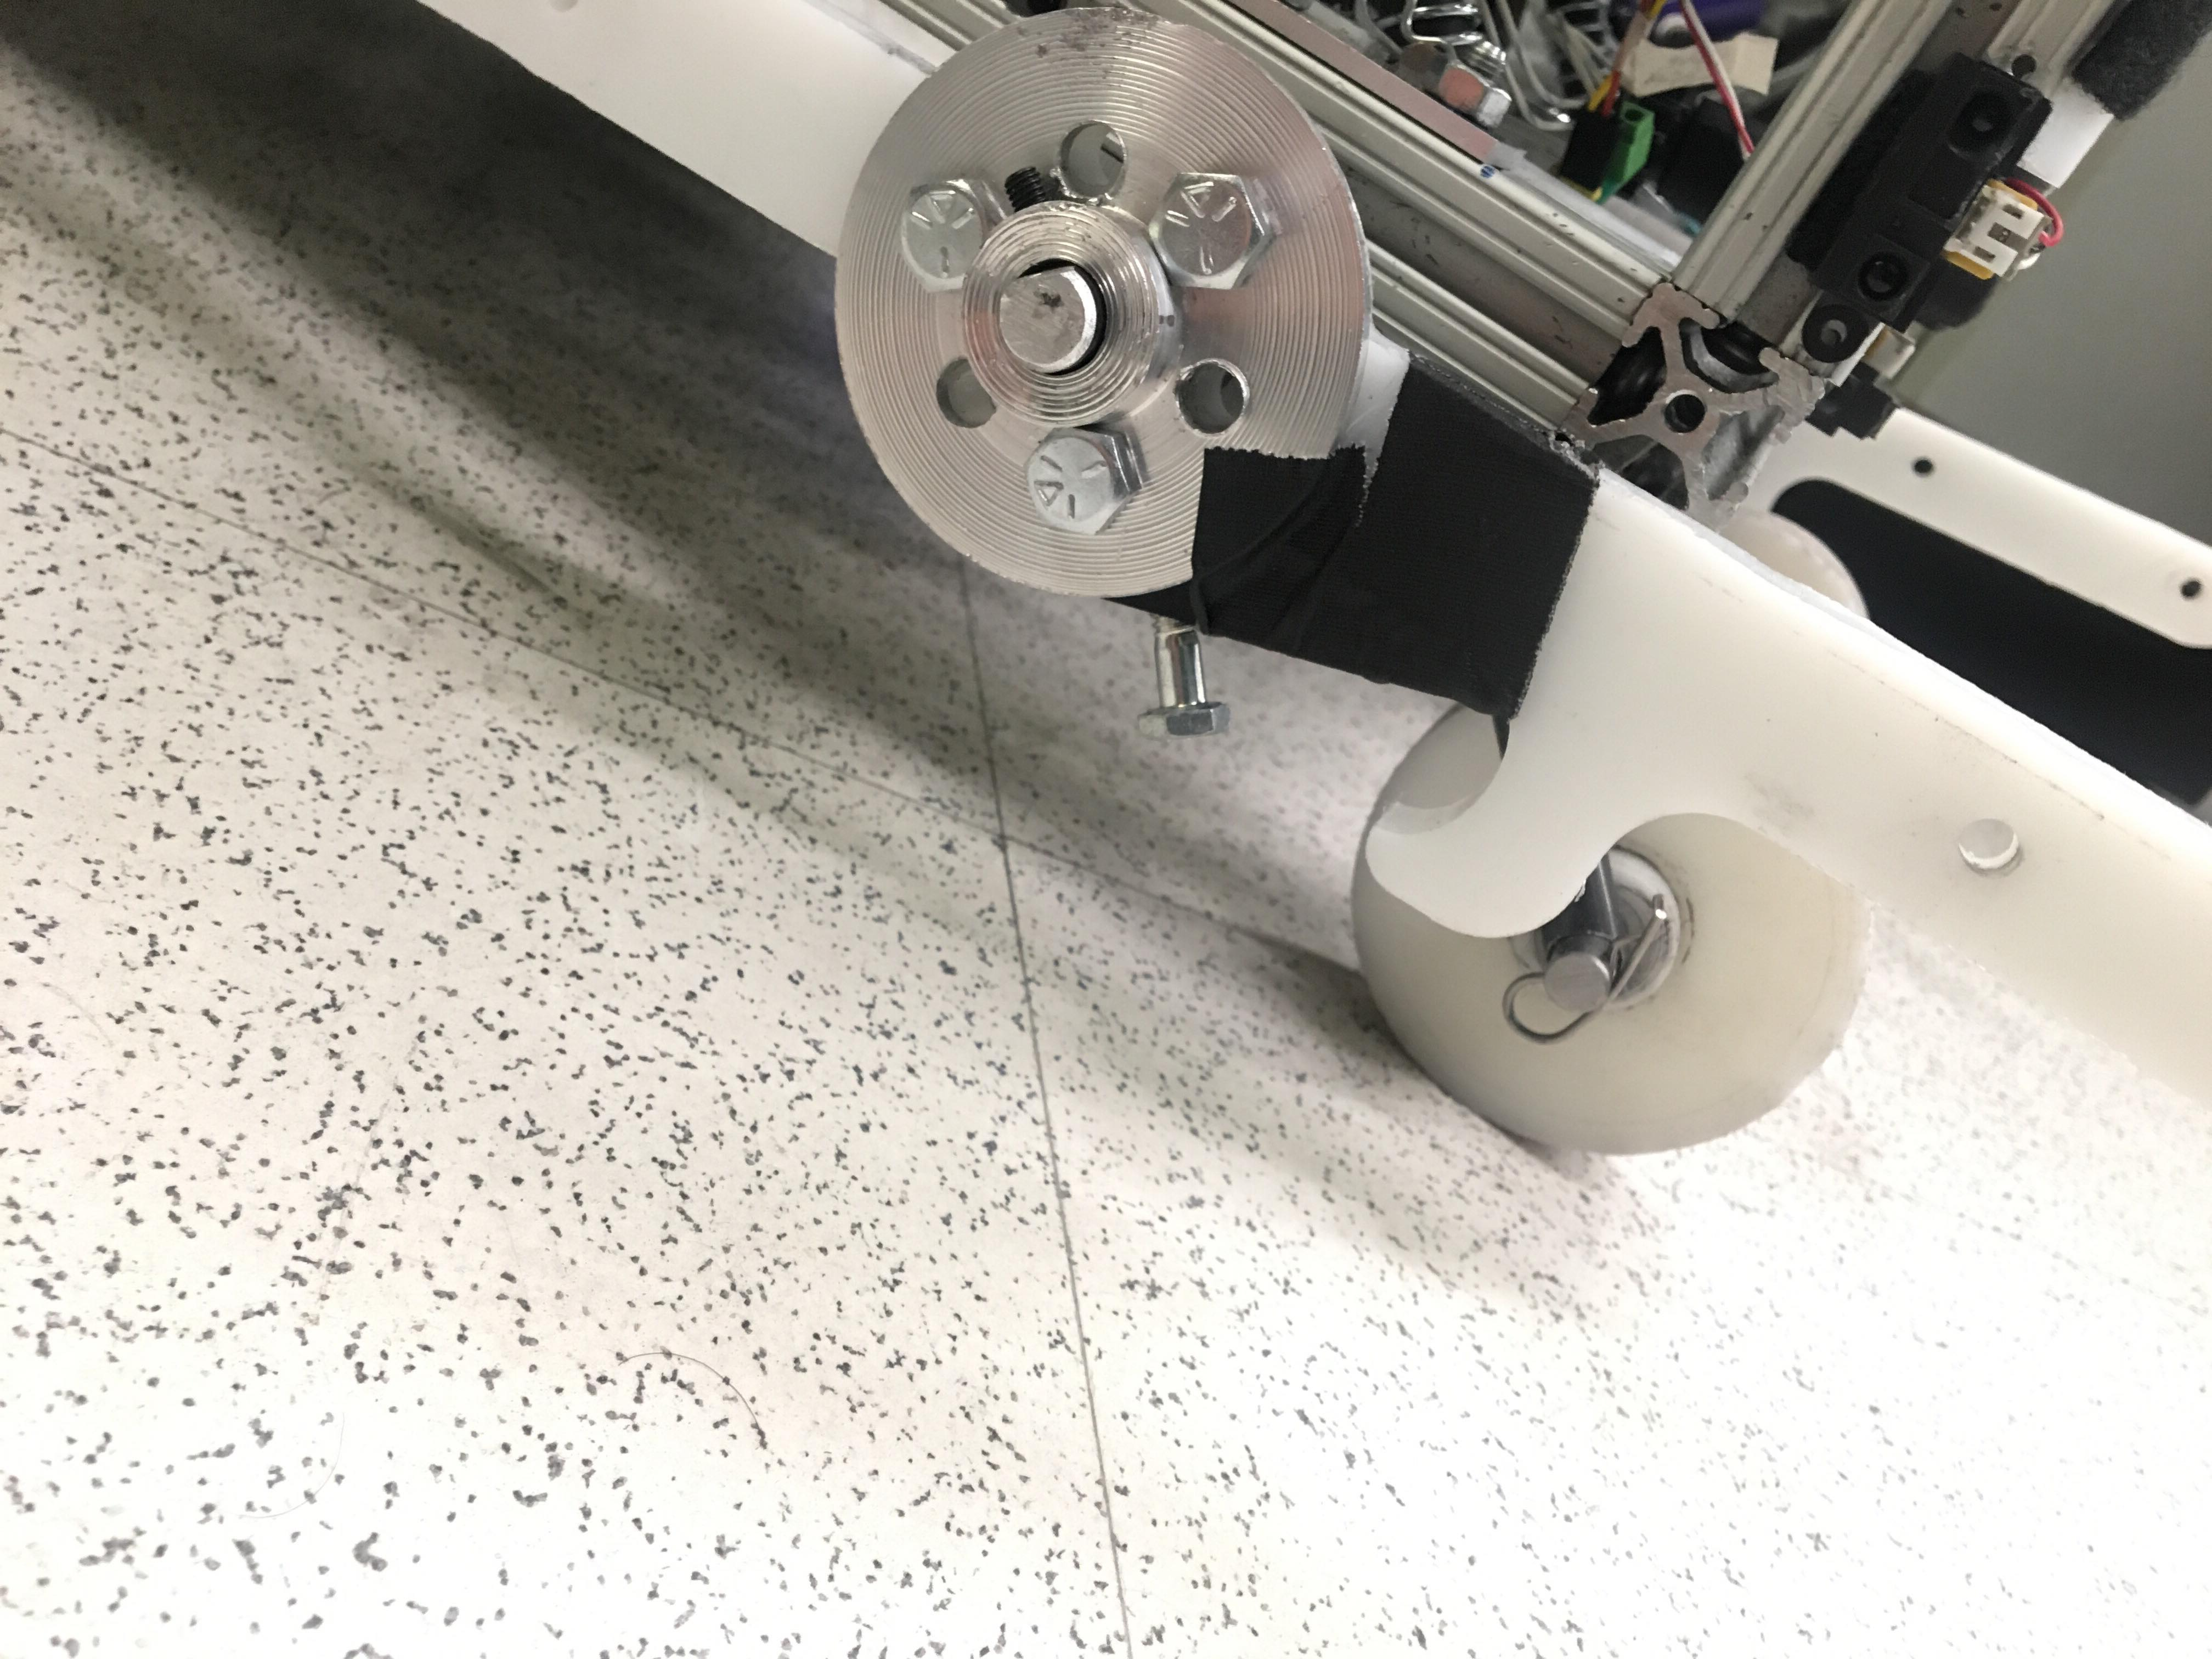
\includegraphics[width=\linewidth]{LiftingArm}
    \caption{Final Lifting Arm Design}
    \label{fig:LiftingArm}
\end{figure}


Having come up with a design for the wall traversal, the SaRRchaeologists also spent time researching other critical design components. From the videos, it became clear that a simple medkit gripper design consisting of a V-shaped protrusion on a rotating arm would be sufficient for picking up and depositing the medkit. It was also clear, however, that the inclusion of a bracket to hold the medkit in place during the course would be necessary in order to prevent it from being dislodged during the violent drop from the wall. A CREO model of the medkit arm is shown in Fig. \ref{fig:MedkitArm}.


The SaRRcheaologists sought to design a SaRR that could not only complete the required tasks, but could do so in an interesting and innovative way that was not reliant on overly complex and failure-prone mechanisms. By iterating through many different geometries for the chassis, front fork assembly, and lifting arms, an innovative, functional design was achieved. In order to maintain the maneuverability of the SaRR through the course, and to keep it from reaching too steep an angle coming off the wall, the chassis was designed to be just long and wide enough to accommodate all the required parts and controlling mechanisms, and no larger. Additionally, emphasis was placed on choosing tires with enough traction and height to aid the SaRR in getting over the wall when working in concert with the lifting arms. Finally, design aspects were chosen to increase the robustness of the SaRR. The frame was designed using 80/20 aluminum extrusion to allow for easy, secure mounting of various components, and to distribute any forces and impulses from the weaker polycarbonate and acrylic sheets to the stronger frame.
The T-slotted 80/20 frame also increased the modularity of the SaRR, so that parts could be moved or replaced with ease. Additionally, in order to reduce the strain on the SaRR each time it dropped off the back of the wall, the front wheels were mounted at a 45 \degree angle to the frame, with shock-absorbing springs mounted onto the supporting forks (Fig. \ref{fig:FrontFork}). The air-filled rear tires were also intended to act as shock absorbers for the back of the robot.

\subsection{Successes and Failures}
As can be expected in any prototyping process, the SaRRchaeologists ran into a number of issues throughout the construction and testing of the robot. One issue that occurred repeatedly involved the shearing of various pins and shafts in the gearboxes. A number of factors contributed to these breakages: severe shocks to the rear wheels upon impact from driving over the walls, and repeated impacts directly to the pins due to imprecise manufacturing that resulted in the side of the gears hitting the pins each time the wheel changed direction. The problem was eventually solved by drilling new holes that were better sized to the pins, and putting in solid dowel pins rather than hollow roll pins.


Additionally, the plastic miter gears initially chosen by the SaRRchaeologists failed after just a few hours of usage, with several of the teeth shearing off completely. Unfortunately, the timing of this failure prevented the team from accomplishing the speed trial milestone on time. After this setback, the team ordered a replacement set of miter gears made of 1144 carbon steel. These miter gears have a yield strength of 620 MPa, and the absolute maximum stress expected on the gears was just under 17 MPa. As expected, these new gears remained completely intact during the usage of the SaRR. These calculations are located in Section \ref{fig:GearStress}.

The SaRRchaeologists where ultimately successful in their attempt to design a sturdy and robust SaRR. Multiple drop tests, as well as accidental inversions during failed autonomous wall traversals proved that the frame of the robot was more than capable of withstanding significant force without breaking or buckling, and the other components were mounted in a way that allowed them to survive large impacts, with only the light sensors mounted to the front of the chassis sustaining damage during an inversion.

An unforeseen problem that the SaRRchaeologists faced was the shifting of the center of gravity going over the wall upon picking up the medkit. Due to the order of the milestones, the lifting arms were designed and tested successfully before the medkit arm assembly was mounted, and while DynaSaRR could easily traverse the wall without the added weight of the medkit, upon picking it up, the weight was shifted too far back and the robot was unable to make it over the final part of the wall, even with the hooks designed for this purpose. A variety of solutions were tested, including adding steel ballast to the front of the robot to shift the center of gravity forward in the hopes of tipping the robot over the wall at the top. Ultimately, success was achieved by adding a bolt to each lifting arm, sitting just in front of the hooks. This bolt levered the circular hub of the arm up, and then slipped forward and caught on the lip of the wall, pulling the robot over as shown in Fig. \ref{fig:bolts}.

Additionally, the SaRRchaeologists had many hardware failures that halted the testing process and adversely affected performance on testing day. The right rear wheel motor (a Vex Mini CIM motor) intermittently stopped responding, but as the problem was seemingly random and difficult to replicate on command, the various fixes attempted (including replacing the snap ring holding the shaft to the gears, replacing the shaft altogether, changing the wires and pins, and replacing the motor controller) failed to reliably fix the problem. It was also difficult to find light and proximity sensors that performed reliably--for example, the day before Demo Day, the SaRRchaeologists noticed that the two light sensors (which had worked well in the past) were reading dramatically different values from each other and did not respond similarly to variations in brightness. This was remedied by testing various sensors and adjusting their variable resistance switches so that they performed more similarly, but the problem was never fully resolved.

Finally, a large unforeseen problem related to the battery life of the drill batteries. The SaRRchaeologists had not initially accounted for not being able to test for extended periods of time due to quick draining of the batteries and poor performance as soon as their level of charge dropped below its peak. This introduced reliability issues in the code--a code that worked at the beginning of testing would have to be adjusted by the end (specifically, the power output to the motors each time the robot was intended to turn had to be increased), as the weaker batteries resulted in drastically different driving performance. However, this new code would then perform poorly the next day on fresh batteries. It appeared that DynaSaRR drained the batteries much faster than expected and performed surprisingly poorly on even half-charged batteries. Were this robot to be improved and rebuilt, managing energy use would be a main concern of the group.

\begin{figure}[ht]
    \centering
    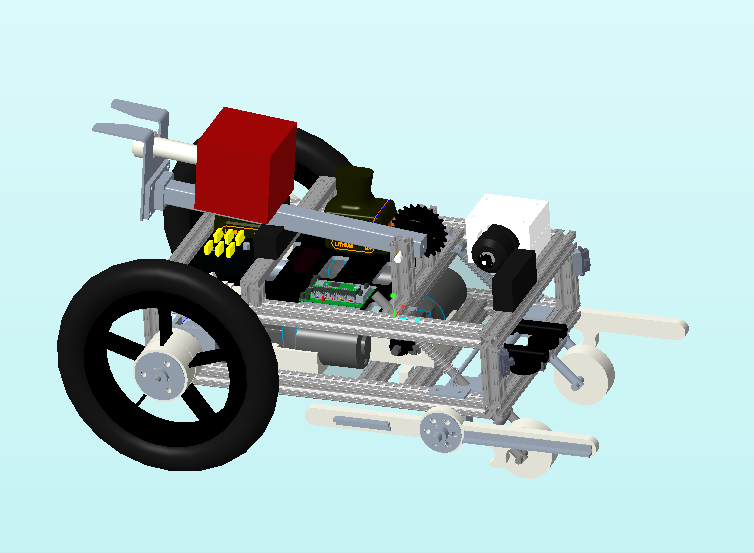
\includegraphics[width=\textwidth]{new_sarr.PNG}
    \caption{DynaSaRR Schematic}
\end{figure}